%\documentclass[conference,a4paper]{IEEEtran}

\documentclass[a4paper]{article}

% Denne linjen vil gjøre livet ditt enklere. Den gjør
% at du kan skrive æøå eller é om du har en sånn teit
% bokstav i navnet ditt.
\usepackage[utf8]{inputenc}

% Denne brukes bare for å få lorem ipsum (tulletekst)
% kjapt opp. På denne måten kan vi se strukturen bedre
\usepackage{blindtext}

% Du må ha denne pakken for å legge inn bilder osv.
\usepackage{graphicx}

% De to neste pakkene tregs dersom du skal ha subfigurer.
\usepackage{caption}
\usepackage{subcaption}

% Denne pakken inneholder mange nyttige måter å skrive
% ligninger på. I tillegg lar den deg droppe equation-nummer
% og sånn.
\usepackage{amsmath}

\begin{document}

\title{Krasj-kurs i \LaTeX}
\author{Andreas Drivenes \& Martin Hallén}
\date{\today}

% Uten denne linjen vil faktisk ingenting av tittelen vises.
% Denne kommandoen tar informasjonen ovenifra og lager en
% fin liten tittel for oss.
\maketitle

% Sammendrag
\begin{abstract}
    \blindtext
\end{abstract}

\section{The basics}

\blindtext

\subsection{Lister}

% Itemize er punktliste. Enumerate er nummerert liste.
\begin{itemize}
    \item Første
    \item Andre
    \begin{itemize}
        \item Underpunkt 1
        \item Underpunkt 2
    \end{itemize}
    \item Tredje
\end{itemize}

\begin{enumerate}
    \item Første
    \item Andre
    \begin{itemize}
        \item Underpunkt 1
        \item Underpunkt 2
    \end{itemize}
    \item Tredje
\end{enumerate}

\subsection{Figurer}

% h sier at figuren skal vises "here", altså der det
% spesifiseres i dokumentet. Du kan velge t (top),
% b (bottom) og p (new page). I tillegg kan du slenge på
% utropstegn for å overskrive det kompilatoren mener er
% beste plassering

% centering vil sette figuren i midten horisontalt.
% caption er det som vil stå under bildet
% label er en unik id som du kan referere til senere

\begin{figure}[h]
    \centering
    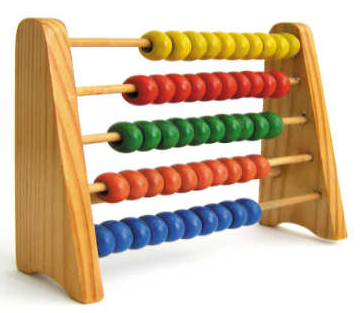
\includegraphics[width=0.5\textwidth]{kuleramme}
    \caption{En sykt bra kuleramme}
    \label{fig:kuleramme}
\end{figure}


\begin{figure}[h]
    \centering
    \begin{subfigure}[b]{0.3\linewidth}
        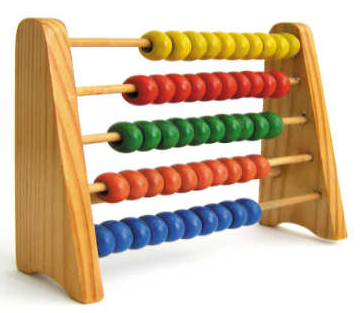
\includegraphics[width=\textwidth]{kuleramme}
        \caption{Ramme 1}
        \label{fig:ramme1}
    \end{subfigure}
    ~ 
    \begin{subfigure}[b]{0.3\linewidth}
        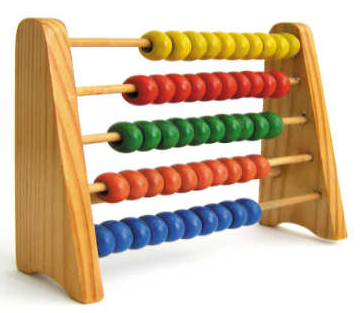
\includegraphics[width=\textwidth]{kuleramme}
        \caption{Ramme 2}
        \label{fig:ramme2}
    \end{subfigure}
    ~ 
    \begin{subfigure}[b]{0.3\linewidth}
        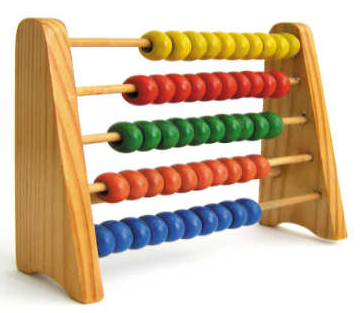
\includegraphics[width=\textwidth]{kuleramme}
        \caption{Ramme 3}
        \label{fig:ramme3}
    \end{subfigure}
    \caption{Tre helt like kulerammer}\label{fig:animals}
\end{figure}

\pagebreak

\subsection{Tabeller}

% \\ sier at det er en ny linje i tabellen
% \hline betyr horisontal linje
% l | c | r betyr at det skal være venstrestilt, midtstilt
% og høyrestilt. Alle sammen med en vertikal strek imellom

\begin{table}[h]
    \centering
    \begin{tabular}{ l | c | r }
      1 & 2 & 3 \\ \hline
      4 & 5 & 6 \\ \hline
      7 & 8 & 9 \\ 
    \end{tabular}
    \caption{Min flotte tabell}
    \label{tab:tabell1}
\end{table}

\begin{table}[h!]
    \centering
    \begin{tabular}{| l | l |}
    \hline
    Speed limit & Basis speed for heavy duty vehicles \\ \hline \hline
    Under 50 km/h & Speed limit \\ \hline
    50 km/h & 56 km/h \\ \hline
    60 km/h & 67 km/h \\ \hline
    70 km/h & 75 km/h \\ \hline
    80 km/h & 80 km/h \\ \hline
    90 km/h & 84 km/h \\ \hline
    \end{tabular}
    \caption{Basis speed for heavy vehicles}
    \label{table:referencespeed}
\end{table}


\subsection{Matematikk}

Kvadratroten er definert som $y = \sqrt{x}$. Dette kan vi skrive inne i teksten.

Vi kan også skrive matte på en ny linje, gjerne hvis den ser stor.

\begin{equation} \label{eq:combinatorics}
    \frac{n!}{k!(n-k)!} = \binom{n}{k}    
\end{equation}

Latex inneholder også enkle måter å lage fine oppsett.

\begin{equation*}
u(x) = 
    \begin{cases} 
        \exp{x} & \text{if } x \geq 0 \\
        1       & \text{if } x < 0
    \end{cases}    
\end{equation*}

Du kan også ha med tekst i ligningen din. Det ser ofte litt dumt ut om du ikke bruker \verb:\text{}:

\begin{equation}
    \text{kuleramme} = 100~\text{kuler} + 1~\text{ramme}
\end{equation}

\subsection{Referanser}

\subsubsection{Referanser i eget dokument}

Du kan se en ganske kul utregning i ligning \ref{eq:combinatorics}, samt masse fin info i tabell \ref{table:referencespeed}. Du kan også spesifisere underfigurer, f.eks. figur \ref{fig:ramme2}.

\subsubsection{Referanser til litteratur}

Alle referanser kan plasseres i en bibtex-fil. Dette gjør det veldig lett å referere til annen litteratur. F.eks. er \cite{tintarev2007survey} en fin kilde om anbefalingssystemer.

\bibliographystyle{unsrt}
\bibliography{references}

\end{document}
